\chapter{GG-Code as a Superset of G-code: Layer-Anchored Editing and Visualization}

\section{Motivation and Scope}

The compilation model presented in Chapter~4 treated GG-Code and G-code as two disjoint languages: GG-Code was the human-readable source, and G-code was the machine-readable output of a one-way translation. While this model is sufficient for authoring new toolpaths from scratch, it breaks down in the most common practical scenario faced by manufacturing engineers and 3D-printing hobbyists, namely the need to take an \emph{existing} machine program, produced by a slicer or a CAM package, and apply a small, targeted modification to it.

Concretely, when a real slicer file --- the reference artefact used throughout this chapter is \texttt{3DBenchy-S3D-Kossel-v3.gcode}, a Simplify3D export of \textbf{142{,}465} lines --- was supplied to the compiler, the ANTLR4 lexer failed on the very first raw motion command. The grammar of Chapter~2 recognises statements such as \texttt{Move to X10 Y20}, but it has no production for a literal \texttt{G1 X10.496 Y-1.648 E0.4346}. The system could therefore neither open nor round-trip the files its users already possessed.

This chapter documents the work undertaken to resolve this limitation by promoting GG-Code from a \emph{translator target} to a strict \textbf{superset} of G-code, and by adding a layer of editing constructs that operate naturally on real, layered machine programs. The intended workflow, agreed with the stakeholders before implementation, is the following:

\begin{enumerate}
    \item A user uploads a \texttt{.gg} \emph{or} a \texttt{.gcode} file. Either opens in the editor as valid GG-Code.
    \item The user inserts code anchored to a position in the print using the constructs \texttt{At layer N \{ \ldots \}} and \texttt{At height H \{ \ldots \}}, or the inline forms \texttt{Pause at layer N} and \texttt{Pause at height H}.
    \item A working \texttt{Pause} command emits a genuine machine pause at the specified metric.
\end{enumerate}

Three design decisions were fixed at the outset and govern the entire chapter. First, the \textbf{representation} of ingested G-code is \emph{hybrid}: raw lines are preserved byte-for-byte (a lossless round-trip), while the compiler additionally injects human-readable navigation annotations. Second, the \textbf{anchoring syntax} provides both a block form and an inline form. Third, the \textbf{Pause} command emits the standard \texttt{M0} host pause, and an anchor that cannot be resolved produces a warning and is skipped rather than aborting the compilation. The remainder of the chapter follows the scientific method: Section~\ref{sec:m3-validation} states the hypotheses that motivated the design and reports the experiments that tested them.

% ─────────────────────────────────────────────────────────────────────────────
\section{From Translator to Superset: An Architectural Shift}

\subsection*{The 142{,}000-line Problem}

The naïve route to a superset would be to extend the grammar with a ``raw G-code line'' production so that every line, whether GG-Code or G-code, flows through the existing five-stage pipeline. This route was rejected on performance grounds. ANTLR4's Python runtime implements the Adaptive LL(*) algorithm as a pure-Python interpreter; constructing a parse tree of several hundred thousand context objects, allocating an AST node per line, and walking the result is prohibitively expensive for files the user expects to open and recompile interactively. An analysis of the reference file is summarised in Table~\ref{tab:benchy-stats}: of its 142{,}465 lines, \textbf{135{,}152} are \texttt{G1} motion commands. Pushing those through the full parser is exactly the cost that must be avoided.

\begin{table}[H]
\centering
\begin{tabular}{|l|r|}
\hline
\textbf{Property} & \textbf{Count} \\
\hline
Total lines & 142{,}465 \\
\texttt{G1} motion commands & 135{,}152 \\
\texttt{G92} resets & 4{,}816 \\
\texttt{M}-codes (temperature, fan, \ldots) & 22 \\
Tool selects (\texttt{T0}) & 1 \\
Layer markers (\texttt{; layer N, Z = h}) & 239 \\
\hline
\end{tabular}
\caption{Composition of the reference Simplify3D file \texttt{3DBenchy-S3D-Kossel-v3.gcode}}
\label{tab:benchy-stats}
\end{table}

\subsection*{Hybrid Line-Oriented Preprocessing}

The adopted solution introduces a \textbf{preprocessor} stage, implemented in \texttt{src/preprocessor/line\_classifier.py}, ahead of the ANTLR4 stages. Its function \texttt{classify\_lines} performs a single linear scan of the source using a small set of pre-compiled regular expressions and assigns every line to one of three categories:

\begin{itemize}
    \item[-] \textbf{Raw G-code} --- a line matching \verb|^\s*[GMT]\d+\b| (a \texttt{G}, \texttt{M}, or \texttt{T} command). It is preserved verbatim.
    \item[-] \textbf{Passthrough comment / blank} --- a line beginning with \texttt{;} or containing no command. It is preserved verbatim. If the comment matches the slicer layer-marker pattern \verb|; layer N, Z = h|, the pair $(N, h)$ is additionally recorded in a layer map.
    \item[-] \textbf{GG-Code DSL} --- a line beginning with a DSL keyword (\texttt{Move}, \texttt{Temperature}, \texttt{Pause}, \texttt{At}, \texttt{Set}, \texttt{Add}, \texttt{If}, \texttt{Repeat}, \ldots) or an opening brace. Only these lines are handed to ANTLR4.
\end{itemize}

Crucially, contiguous runs of raw and comment lines are coalesced into a \emph{single} node, broken only at layer markers. The 142{,}465-line reference file thus collapses to a few hundred nodes rather than one node per line. Lines that open a brace-delimited block (\texttt{At layer 5 \{}) are accumulated, with brace-balance tracking, into one DSL chunk so that multi-line constructs reach the parser intact.

\subsection*{The \texttt{RawGCode} Node and Verbatim Fidelity}

Raw and comment runs are represented by a new AST node, \texttt{RawGCode}, defined in \texttt{src/ast\_nodes/statements.py}:

\begin{verbatim}
@dataclass
class RawGCode(Statement):
    text: str                      # the verbatim line(s)
    layer: Optional[int] = None
    z: Optional[float] = None
    is_layer_marker: bool = False
\end{verbatim}

Because an unrecognised line is emitted exactly as received, the superset property holds \emph{by construction}: any line the preprocessor does not recognise as DSL is preserved without reformatting. The code generator emits a \texttt{RawGCode} node's text directly, and for layer-marker nodes additionally emits a friendly annotation such as \verb|; >> Layer 5 (Z=1.100mm)|, realising the hybrid representation.

This division of labour --- raw lines on a fast verbatim path, only the small DSL portion through ANTLR4 --- preserves the academic value of the parser while making the system usable on production files. The revised pipeline is shown in Figure~\ref{fig:m3-pipeline}.

\begin{figure}[H]
\centering
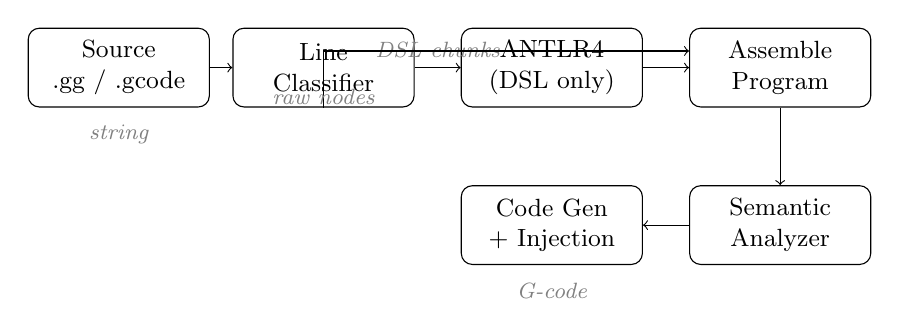
\begin{tikzpicture}[
  node distance=2.6cm,
  box/.style={draw, rounded corners, minimum width=2.3cm, minimum height=1.0cm, align=center, font=\small},
  note/.style={font=\footnotesize\itshape, text=gray}
]
\node[box] (src)  {Source\\.gg / .gcode};
\node[box] (pre)  [right of=src] {Line\\Classifier};
\node[box] (ant)  [right of=pre, node distance=2.9cm] {ANTLR4\\(DSL only)};
\node[box] (asm)  [right of=ant, node distance=2.9cm] {Assemble\\Program};
\node[box] (sem)  [below of=asm, node distance=2.0cm] {Semantic\\Analyzer};
\node[box] (gen)  [left of=sem, node distance=2.9cm] {Code Gen\\+ Injection};

\draw[->] (src) -- (pre);
\draw[->] (pre) -- node[note, above]{DSL chunks} (ant);
\draw[->] (ant) -- (asm);
\draw[->] (pre.south) |- ([yshift=6pt]asm.west) node[note, below, pos=0.25]{raw nodes};
\draw[->] (asm) -- (sem);
\draw[->] (sem) -- (gen);

\node[note] at (src.south)  [below=0.1cm] {string};
\node[note] at (gen.south)  [below=0.1cm] {G-code};
\end{tikzpicture}
\caption{Revised pipeline. Raw lines bypass ANTLR4 and are interleaved with parsed DSL statements in source order; the generator resolves anchors during code generation.}
\label{fig:m3-pipeline}
\end{figure}

% ─────────────────────────────────────────────────────────────────────────────
\section{Layer and Height Anchoring}

\subsection*{Grammar Extensions}

Three additions were made to \texttt{src/grammar/GGCode.g4}. A new keyword token \texttt{HEIGHT} was introduced, an \texttt{anchorTarget} rule expresses the two anchor flavours, and the \texttt{pauseStatement} rule was generalised. The relevant productions are:

\begin{verbatim}
pauseStatement   : PAUSE (AT anchorTarget)? ;
anchorTarget     : LAYER INTERGER   # layerAnchor
                 | HEIGHT measure   # heightAnchor ;
atBlockStatement : AT anchorTarget blockStatement ;
\end{verbatim}

The \texttt{atBlockStatement} production was wired into \texttt{compoundStatement} alongside the existing conditional, loop, and block constructs. A defensive lexer rule \verb|GCODE_COMMENT: ';' ~[\r\n]* -> skip| was also added so that any \texttt{;}-style comment surviving inside a DSL chunk is harmlessly discarded rather than causing a parse failure. The deliberate spelling \texttt{INTERGER} of the integer token, established in Chapter~2, was preserved for consistency. After editing the grammar, the parser was regenerated with the ANTLR4 tool-jar as described in Section~3.1.

\subsection*{New AST Nodes}

The anchoring constructs are represented by two new node types and a small value object:

\begin{verbatim}
@dataclass
class Anchor:                       # value object, not a Statement
    kind: str                       # 'layer' | 'height'
    layer: Optional[int] = None
    height: Optional[float] = None  # millimetres

@dataclass
class AtBlockStatement(Statement):
    anchor: Anchor
    body: Block

@dataclass
class PauseStatement(Statement):
    anchor: Optional[Anchor] = None  # None => inline pause
\end{verbatim}

The corresponding visitor methods \texttt{visitLayerAnchor}, \texttt{visitHeightAnchor}, \texttt{visitAtBlockStatement}, and \texttt{visitPauseStatement} were added to \texttt{ASTBuilder}. Height anchors are normalised to millimetres at construction time, so \texttt{2cm} and \texttt{20mm} produce identical \texttt{Anchor} objects.

\subsection*{The \texttt{Pause} Command: A Latent-Bug Fix}

The work in this chapter also corrected a defect inherited from the original implementation. The grammar of Chapter~2 contained a \texttt{pauseStatement} production, but \texttt{ASTBuilder} provided no \texttt{visitPauseStatement} override. Consequently every \texttt{Pause} statement was silently discarded by the default visitor, and no pause ever reached the generated output. Supplying the visitor, together with the generalised grammar, makes \texttt{Pause} a first-class, working command for the first time: a bare \texttt{Pause} now emits an inline \texttt{M0}, and the anchored forms are injected at the resolved position (Section~\ref{sec:m3-injection}).

\subsection*{Semantic Treatment}

The semantic analyzer was extended to recognise the new nodes. \texttt{RawGCode} is treated as opaque and passes validation unconditionally, since its content is verbatim machine code outside the language's semantic model. \texttt{AtBlockStatement} has its body analysed recursively and its anchor structurally validated (a layer index must be non-negative; a height must be strictly positive). The question of whether an anchored layer or height \emph{exists} in a given file is deliberately \emph{not} answered here: that fact is only known once the layer map has been resolved during code generation, and is reported there as a warning rather than a fatal error, in keeping with the design decision that a missing anchor must never abort a compile.

% ─────────────────────────────────────────────────────────────────────────────
\section{Two-Pass Code Generation with Injection}
\label{sec:m3-injection}

Anchored constructs introduce a non-local dependency: an \texttt{At layer 50} block written at the end of the source must emit its output near the \emph{middle} of the generated file. The code generator therefore adopts a two-pass strategy, illustrated in Figure~\ref{fig:m3-injection}.

In \textbf{Pass~A}, the generator walks the program in source order and emits the base output. As it does so it records, for each layer, the index in the output line list at which that layer begins (\texttt{layer\_anchors}), and maintains a list of $(z, \text{index})$ pairs for height resolution (\texttt{z\_anchors}). Anchors are registered both at \texttt{RawGCode} layer-marker nodes and at Z-axis moves emitted by DSL \texttt{Move} statements, so the mechanism works for fully raw files, fully authored files, and mixtures of the two. When the walk encounters an \texttt{AtBlockStatement} or an anchored \texttt{PauseStatement}, it does \emph{not} emit inline; instead it renders the construct's body into an isolated line list and appends the pair (anchor, lines) to an injection table.

In \textbf{Pass~B}, each injection's anchor is resolved to an output index --- a layer anchor maps directly through \texttt{layer\_anchors}; a height anchor maps to the first recorded $z \geq H$ --- and the rendered lines are spliced in. The splices are applied in \emph{descending} index order so that an earlier insertion does not invalidate the indices of later ones. If an anchor cannot be resolved, a message is appended to a warnings list, surfaced both on standard error and as a \verb|; WARNING:| comment near the top of the output, and the injection is skipped.

\begin{figure}[H]
\centering
\begin{tikzpicture}[
  node distance=1.0cm and 1.4cm,
  box/.style={draw, rounded corners, minimum width=3.0cm, minimum height=0.9cm, align=center, font=\small},
  small/.style={font=\footnotesize}
]
\node[box] (walk) {Pass A: walk program};
\node[box, below=of walk] (rec) {record layer / z anchors};
\node[box, right=of walk] (coll) {collect anchored\\blocks (deferred)};
\node[box, below=of rec] (res) {Pass B: resolve anchors};
\node[box, below=of res] (spl) {splice (descending index)};
\node[box, right=of spl] (warn) {unresolved $\rightarrow$ warning};

\draw[->] (walk) -- (rec);
\draw[->] (walk) -- (coll);
\draw[->] (rec) -- (res);
\draw[->] (coll) |- (res);
\draw[->] (res) -- (spl);
\draw[->] (res) -- (warn);
\end{tikzpicture}
\caption{Two-pass injection. Pass~A emits the base output and records anchors; Pass~B splices deferred blocks at their resolved positions.}
\label{fig:m3-injection}
\end{figure}

\paragraph{A note on chunk unwrapping.}
Because each DSL chunk is parsed independently, \texttt{visitProgram} wraps a chunk's statements in a single \texttt{Block}. The helper \texttt{\_parse\_dsl\_chunk} in \texttt{src/main.py} unwraps this outer block so that top-level anchored constructs sit directly in the program's statement list, where the generator's injection routing can see them. Without this step the constructs would be nested one level too deep and would be emitted inline rather than injected --- a subtlety that was diagnosed and corrected during development.

\subsection*{Worked Example}

Given the following input, in which a raw three-layer file is augmented with one anchored block and one anchored pause:

\begin{verbatim}
; layer 1, Z = 0.300
G1 X1 Y1 E0.1
; layer 2, Z = 0.500
G1 X2 Y2 E0.2
; layer 3, Z = 0.700
G1 X3 Y3 E0.3
At layer 2 { Temperature 180C }
Pause at height 0.6mm
\end{verbatim}

the compiler produces the following output. The \texttt{At layer 2} block is injected immediately after the layer-2 boundary, and the height anchor \texttt{0.6mm} resolves to layer~3 (the first layer reaching $Z \geq 0.6$):

\begin{verbatim}
; Start of GG-Code Program
; layer 1, Z = 0.300
; >> Layer 1 (Z=0.300mm)
G1 X1 Y1 E0.1
; layer 2, Z = 0.500
; >> Layer 2 (Z=0.500mm)
M104 S180 ; Set Temp
G1 X2 Y2 E0.2
; layer 3, Z = 0.700
; >> Layer 3 (Z=0.700mm)
; PAUSE at height 0.6mm
M0
G1 X3 Y3 E0.3
; End of Program
\end{verbatim}

% ─────────────────────────────────────────────────────────────────────────────
\section{Revised Module Structure}

The changes add one module and revise three others. Table~\ref{tab:m3-files} lists the components touched in this phase, complementing the project structure of Section~4.1.

\begin{table}[H]
\centering
\begin{tabular}{|l|p{8.7cm}|}
\hline
\textbf{File / Directory} & \textbf{Change} \\
\hline
\texttt{src/preprocessor/line\_classifier.py} & \textbf{New.} Classifies source lines and builds the layer map; emits \texttt{RawGCode} run-nodes and DSL chunks \\
\hline
\texttt{src/grammar/GGCode.g4} & \texttt{HEIGHT} token; \texttt{anchorTarget}, \texttt{atBlockStatement}; generalised \texttt{pauseStatement}; defensive \texttt{;}-comment rule \\
\hline
\texttt{src/ast\_nodes/statements.py} & New \texttt{RawGCode}, \texttt{Anchor}, \texttt{AtBlockStatement}; redefined \texttt{PauseStatement} \\
\hline
\texttt{src/parser/antlr\_converter.py} & \texttt{visitPauseStatement}, \texttt{visitAtBlockStatement}, \texttt{visitLayerAnchor}, \texttt{visitHeightAnchor} \\
\hline
\texttt{src/main.py} & \texttt{run\_pipeline} rewired to classify-then-parse; \texttt{\_parse\_dsl\_chunk} helper \\
\hline
\texttt{src/codegen/gcode\_generator.py} & Two-pass generation with anchor recording, injection, and warnings; verbatim \texttt{RawGCode} emission \\
\hline
\texttt{src/semantic/semantic\_analyzer.py} & Validation for \texttt{RawGCode}, \texttt{AtBlockStatement}, and the new \texttt{PauseStatement} \\
\hline
\texttt{frontend/src/components/GCodeVisualizer.tsx} & Pause surfaces, layer slider, per-layer segmentation \\
\hline
\texttt{tests/test\_gcode\_superset.py} & \textbf{New.} Hypothesis-driven test suite (Section~\ref{sec:m3-validation}) \\
\hline
\end{tabular}
\caption{Modules added or revised in the superset extension}
\label{tab:m3-files}
\end{table}

% ─────────────────────────────────────────────────────────────────────────────
\section{Web IDE Enhancements}

\subsection*{Opening \texttt{.gcode} as GG-Code}

The Monaco-based editor was given a second syntax-highlighting language, \texttt{gcode}, whose tokenizer colours \texttt{G}/\texttt{M} commands, tool selects, axis and feedrate parameters, and \texttt{;} comments. When a file is uploaded, its extension is inspected: a \texttt{.gcode} file activates the \texttt{gcode} language, while a \texttt{.gg} file (or a built-in sample) uses the existing \texttt{ggcode} language. The \texttt{ggcode} tokenizer was also extended with the \texttt{HEIGHT} keyword and \texttt{mm}/\texttt{cm} measure literals introduced for anchoring. The backend required no change, as the \texttt{/upload} endpoint already returns raw file contents.

\subsection*{Visualizing Pauses}

The Three.js visualizer was extended to make pauses visible in three dimensions. The G-code parser, which previously tracked only motion, now also tracks the active layer height (from \verb|; layer| markers, the \verb|; >> Layer| annotations, and Z moves) and detects the \verb|; PAUSE| comments emitted by the generator. A checkbox toggle, ``Highlight pauses'', controls two effects: every toolpath segment on a paused layer is recoloured, and a translucent horizontal \emph{surface} is drawn across the full extent of each paused layer at its $Z$ height. The surface --- sized to the layer's own XY bounding box, with a small overhang --- communicates ``the print pauses here'' far more legibly than a point marker would.

\subsection*{The Layer Slider}

A slider ranging from $0$ to the total layer count controls how many layers, counted from the bottom upward, are rendered. This lets the user peel the model back one layer at a time to inspect interior structure and to confirm where an anchored block was injected. The paused layers are marked as ticks on the slider track at their corresponding positions, tying the temporal notion of a pause to the spatial layer-selection control.

\subsection*{A Segmentation Defect and Its Resolution}

Implementing the slider exposed a latent defect in the visualizer's path parser. The parser began a new render segment only when the G-code command \emph{type} changed between \texttt{G0} (rapid) and \texttt{G1} (linear). Real slicer output, including the reference file, frequently uses \texttt{G1} exclusively; no command change ever occurred, so the entire model collapsed into a single segment tagged with the topmost layer. The slider consequently hid the whole model except at its maximum value. The fix was to break a segment whenever the \emph{layer} changes --- on a Z move or a layer marker --- in addition to command changes. On the reference file this yields 241 segments across all 241 layers, and the slider behaves as intended.

% ─────────────────────────────────────────────────────────────────────────────
\section{Validation: A Hypothesis-Driven Evaluation}
\label{sec:m3-validation}

The extension was developed and assessed using an explicitly hypothesis-driven method. Five hypotheses were stated before implementation, each paired with an experiment, and the resulting test suite (\texttt{tests/test\_gcode\_superset.py}) encodes those experiments as automated checks. Table~\ref{tab:m3-hypotheses} summarises the hypotheses and outcomes.

\begin{table}[H]
\centering
\begin{tabular}{|c|p{6.0cm}|p{4.6cm}|}
\hline
\textbf{H} & \textbf{Hypothesis} & \textbf{Outcome} \\
\hline
H1 & Any raw G-code line is carried through unchanged (superset fidelity). & Confirmed: all 135{,}152 \texttt{G1} lines and every \texttt{G92}/\texttt{M}/\texttt{T} command preserved 1:1. \\
\hline
H2 & Routing only DSL through ANTLR4 keeps large files interactive. & Confirmed: 142{,}465 lines compile in $\approx 0.15$\,s. \\
\hline
H3 & \texttt{At layer/height} blocks inject at the correct position. & Confirmed by placement assertions. \\
\hline
H4 & \texttt{Pause} works end-to-end (no longer dropped). & Confirmed: regression and placement tests pass. \\
\hline
H5 & A missing anchor degrades gracefully. & Confirmed: warning emitted, compile succeeds. \\
\hline
\end{tabular}
\caption{Hypotheses and validation outcomes for the superset extension}
\label{tab:m3-hypotheses}
\end{table}

The decisive result is H2. The reference file of 142{,}465 lines compiles end-to-end in approximately $0.15$~seconds, against a target of ten seconds, while conserving the exact count of every machine command (H1). The full suite of \textbf{22} tests --- the ten pre-existing pipeline tests plus twelve new ones covering verbatim fidelity, layer-marker detection, block and inline injection placement, unit conversion (\texttt{2cm} $\rightarrow$ 20\,mm), the pause regression, mixed ordering, the missing-anchor warning, and a large-file performance check --- passes. As an end-to-end confirmation, appending \texttt{At layer 50 \{ Pause \}} to the reference file injects exactly one \texttt{M0}, positioned immediately after the \texttt{; layer 50} marker.

% ─────────────────────────────────────────────────────────────────────────────
\section{Updated Limitations and Future Work}

This phase resolves two items previously identified in Section~\ref{sec:limitations}. The \texttt{Pause} command, formerly inert, is now fully functional, and the compiler can ingest and round-trip arbitrary G-code rather than only programs authored in GG-Code. Several limitations remain or are newly introduced by the extension.

\paragraph{Height resolution is layer-granular.}
A height anchor resolves to the first layer whose $Z$ reaches the requested value; it cannot inject \emph{within} a layer. This matches the granularity at which pauses are physically meaningful in layered manufacturing, but it means \texttt{At height 2.45mm} on a 0.2\,mm-layer print snaps to the layer boundary at $Z = 2.6$ rather than interpolating.

\paragraph{Absolute-coordinate assumption.}
Both the layer tracker and the visualizer interpret coordinates as absolute (\texttt{G90}). A file that switches to relative mode (\texttt{G91}) would mislead the layer-detection logic. Honouring the modal \texttt{G90}/\texttt{G91} state is a natural next step.

\paragraph{Arc moves are not visualized as layers.}
The visualizer tracks layers from linear (\texttt{G0}/\texttt{G1}) moves; arc commands (\texttt{G2}/\texttt{G3}) are not yet decomposed for layer attribution, so CNC programs dominated by arcs would under-report their layer structure.

\paragraph{Toward conditional anchoring.}
A compelling extension is to allow anchored blocks to carry conditions evaluated against print metadata (for example, ``insert a purge only on layers that change tool''). This would build directly on the injection machinery introduced here, combining it with the static-evaluation model of Chapter~4.
